\chapter{Estado del arte}
\label{cap:capitulo2}

\begin{flushright}
\begin{minipage}[]{10cm}
\emph{Todo progreso depende de la irracionalidad del hombre razonable.}\\
\end{minipage}\\

George Bernard Shaw\\
\end{flushright}

\vspace{1cm}

En el presente capítulo se van a describir algunos de los prototipos y posibles aplicaciones más destacables sobre la detección y mantenimiento del pavimento de las carreteras usando inteligencia artificial y técnicas robóticas. En este estado del arte, se revisan cuatro soluciones tecnológicas innovadoras desarrolladas recientemente: el sistema robotizado basado en \textit{Raspberry Pi} para la reconstrucción 3D de baches (Infrarob), el Proyecto HERON para el mantenimiento robótico de carreteras, la plataforma EyesNroad para la detección de deterioros viales mediante \ac{IA}, y el proyecto OMICRON para la automatización del sellado de grietas.


\subsubsection{Sistema robotizado basado en Raspberry Pi para la reconstrucción 3D de baches}

\setcounter{footnote}{25} 
Este sistema explicado en \cite{s23135860}, es creado como parte del proyecto Infrarob\footnote{\url{https://infrarobproject.com/}} y desarrollado en el marco del proyecto europeo Horizon 2020, utiliza una \textit{Raspberry Pi 4B} acoplada a un robot autónomo para capturar imágenes usando una cámara y coordenadas \acs{GPS}, usando el módulo  de baches en carreteras. Las imágenes, tomadas desde diferentes ángulos, son procesadas mediante técnicas fotogramétricas para generar modelos 3D de los baches, permitiendo calcular con precisión el volumen que debe ser rellenado. El sistema también integra un \ac{SIG} para mejorar la gestión del mantenimiento de pavimentos. (Figura \ref{fig:infrarob})

\begin{figure} [h!]
	\begin{center}
		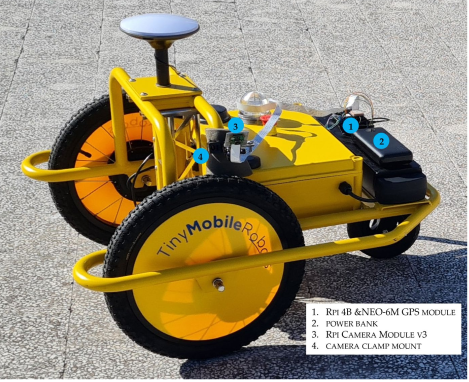
\includegraphics[width=16cm]{figs/infrarob.png}
	\end{center}
	\caption{Robot usado para la reconstrucción 3D de baches}
\label{fig:infrarob}
\end{figure}

Las ventajas de este proyecto son las siguientes: 
\begin{itemize}
	\item \textit{Bajo costo}. Utiliza componentes de bajo costo como: \textit{Raspberry pi}, \textit{Raspberry pi camera} y el módulo \textit{GPS NEO-6M} que también es \textit{low-cost}. 
	\item \textit{Precisión en la detección}. Capacidad para detectar baches de hasta 75 cm de diámetro y crear modelos 3D precisos.
	\item \textit{Integración con \acs{SIG}}. Facilita la planificación de reparaciones.
	
\end{itemize}\


Las desventajas de este proyecto son las siguientes: 
\begin{itemize}
	\item \textit{Limitaciones climáticas}. No puede operar en condiciones adversas ni durante la noche.
	\item \textit{Uso de software de pago}. Utiliza \textit{ContextCapture}, que es de pago, para el procesamiento fotogramétrico.
	\item \textit{Movimiento circular para detección del volumen}. Una vez detectado el bache, es necesario moverse alrededor de él para que el algoritmo de fotogametría sea capaz de encontrar su volumen, lo que ralentiza el cálculo.
	
\end{itemize}\

\subsubsection{El proyecto Herón}

En \cite{10.1145/3529190.3534746} se habla del Proyecto HERON\footnote{\url{https://www.heron-h2020.eu/}}, también parte del programa Horizon 2020, propone una solución integral para el mantenimiento de infraestructuras viales mediante el uso de vehículos modulares robóticos autónomos y drones. El sistema está diseñado para optimizar la eficiencia y seguridad de las operaciones de mantenimiento, utilizando sensores y escáneres para crear mapas 3D, inteligencia artificial para coordinar flujos de trabajo, y módulos de análisis de imágenes para detectar defectos. Todavía está en etapa de desarrollo. (Figura \ref{fig:heron})


\begin{figure} [h!]
	\begin{center}
		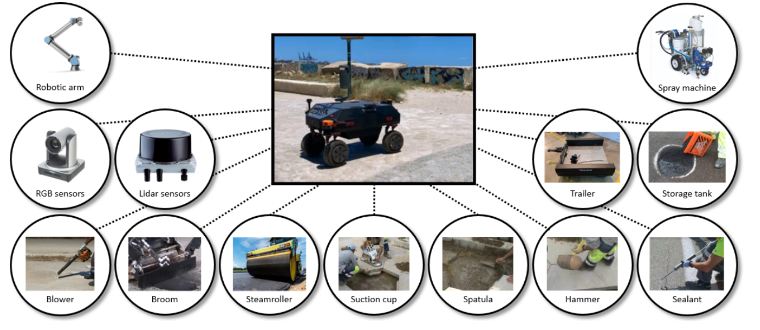
\includegraphics[width=16cm]{figs/heron.png}
	\end{center}
	\caption{Proyecto HERON}
	\label{fig:heron}
\end{figure}

Las ventajas de este proyecto son las siguientes:

\begin{itemize}
	\item \textit{Automatización completa}. Minimiza la intervención humana y reduce riesgos laborales.
	\item \textit{Eficiencia}. El objetivo es mejorar la capacidad y eficiencia de las redes viales.
	\item \textit{Intercambio de datos en tiempo real}. Otro de los objetivos es mejorar la toma de decisiones
	\item \textit{Diseño modular}. Para poder maximizar sus capacidades, facilitar el transporte y reducir los costos de mantenimiento y accidentes.
\end{itemize}\

Las desventajas de este proyecto son las siguientes:
\begin{itemize}
	\item \textit{Costo inicial elevado}. La implementación de tecnologías avanzadas es costosa.
	\item \textit{Dependencia tecnológica}. Requiere una infraestructura tecnológica robusta para su funcionamiento.
\end{itemize}\


\subsubsection{EyesNroad}

EyesNroad es una plataforma que emplea \ac{IA} y \textit{Machine Learning} para identificar baches, señalización y otros deterioros en carreteras a partir de videos capturados por cámaras georreferenciadas instaladas en vehículos. La plataforma genera inventarios detallados y reportes del estado de las carreteras, facilitando el control y mantenimiento de las mismas. Esta aplicación ha sido desarrollada para participar en los XX premios de conservación de carreteras de \ac{ACEX} (año 2024)\footnote{\url{https://www.acex.eu/candidatura-3-4/}} que ha resultado ganadora en la en la categoría general. Puedes ver su aspecto en la Figura \ref{fig:enr}.

\begin{figure} [h!]
	\begin{center}
		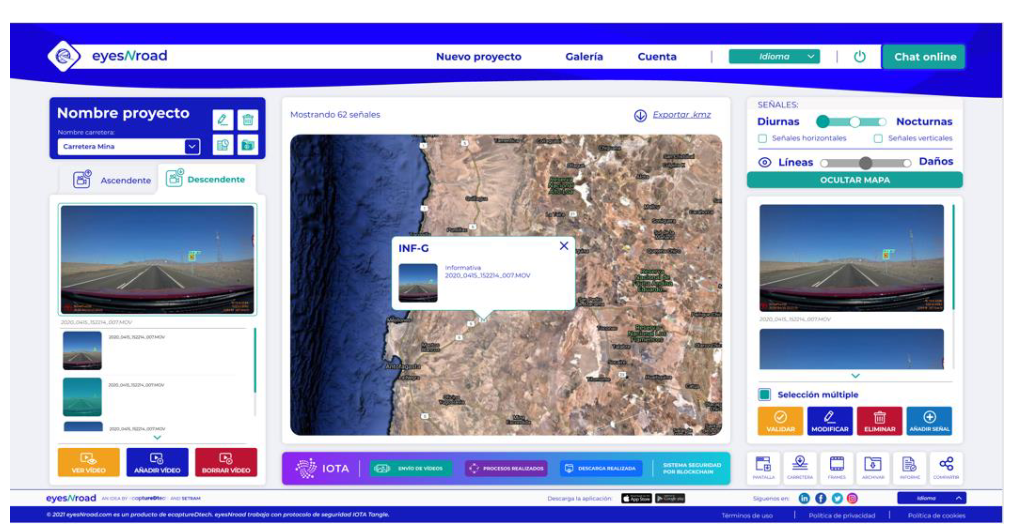
\includegraphics[width=16cm]{figs/enr.png}
	\end{center}
	\caption{Visualización de la señal en un mapa en eyesNroad}
	\label{fig:enr}
\end{figure}


Las ventajas de este proyecto son las siguientes:

\begin{itemize}
	\item \textit{Facilidad de implementación}. Puede utilizarse con cámaras comunes y es compatible con dispositivos móviles.
	\item \textit{Amplia detección}. No solo identifica baches, sino también señalización y otros elementos viales.
	\item \textit{Actualización continua}. La base de datos se amplía constantemente para cubrir más regiones.
	
\end{itemize}\

Las desventajas de este proyecto son las siguientes:
\begin{itemize}
	\item \textit{Limitación geográfica}. Actualmente, su funcionamiento completo está limitado a Portugal.
	\item \textit{Es de pago}. Para cualquier persona que desee usar esta herramienta tiene que asumir los costes.
	\item \textit{No calcula volumen}. La plataforma no ofrece estimaciones del volumen de los baches, lo que podría ser útil para reparaciones.
	
\end{itemize}\


\subsubsection{El proyecto OMICRÓN}

Dentro del proyecto OMICRON se ha decidido crear un sistema robótico que busca automatizar y robotizar el proceso de sellado de grietas en pavimentos, con el objetivo de eliminar la exposición de los operarios a condiciones peligrosas. El sistema integra un brazo robótico y herramientas de inteligencia artificial para detectar grietas y realizar el sellado de manera autónoma, mejorando así la seguridad y eficiencia en las operaciones de mantenimiento. Esta aplicación ha sido desarrollada para participar en los XX premios de conservación de carreteras de \ac{ACEX} (año 2024)\footnote{\url{https://www.acex.eu/candidatura-12-5/}} que ha resultado ganadora en la en la categoría asociados. Puedes ver su aspecto en la Figura \ref{fig:omicron}.

\begin{figure} [h!]
	\begin{center}
		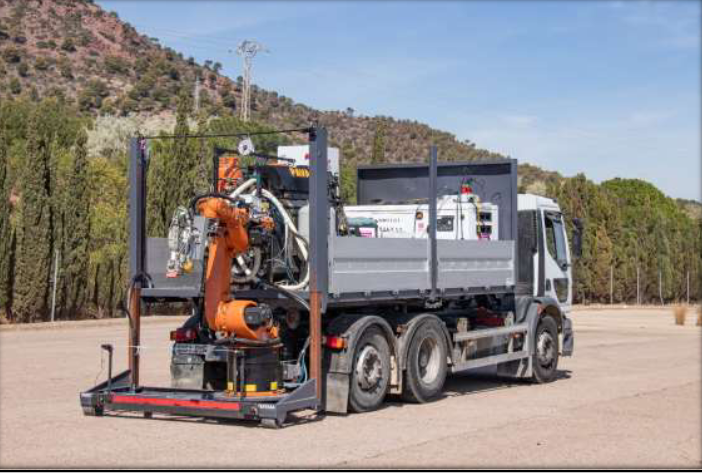
\includegraphics[width=16cm]{figs/omicron.png}
	\end{center}
	\caption{Plataforma robótica diseñada para el sellado de grietas}
	\label{fig:omicron}
\end{figure}

Las ventajas de este proyecto son las siguientes:

\begin{itemize}
	\item \textit{Seguridad laboral}. Elimina la necesidad de que los operarios sufran accidentes de tráfico y tengan contacto con materiales peligrosos.
	\item \textit{Reducción de tiempo}. Debido a la automatización del proceso, se puede reducir el tiempo de intervención.
	\item \textit{Innovación en materiales}. Al invertir en crear un mástico nuevo, se puede operar a temperaturas más bajas.
\end{itemize}\


Las desventajas de este proyecto son las siguientes:

\begin{itemize}
	\item \textit{Es un prototipo}. Todavía está en fase temprana de implementación lo que le impide a los clientes tener una disponbilidad inmediata.
	\item \textit{Alto costo}. Necesita componentes caros para poder llevar a cabo sus objetivos: un camión, un brazo robótico, entre otros.
	\item \textit{Complejidad técnica}. Ya que se trata de una automatización completa, necesita un alto nivel de precisión y coordinación, supone un gran desafío para su implementación.
\end{itemize}\


Los prototipos y desarrollos tecnológicos presentados demuestran el potencial de la robótica y la inteligencia artificial en el mantenimiento y detección de deterioros en el pavimento. Desde la creación de modelos 3D de baches hasta la automatización del sellado de grietas, estos avances no solo mejoran la seguridad y eficiencia de las operaciones, sino que también optimizan la gestión y planificación del mantenimiento vial. No obstante, cada solución presenta desafíos específicos, como la dependencia de condiciones climáticas, la limitación geográfica y los costos asociados, que deben ser considerados al evaluar su implementación en diferentes contextos. En el siguiente capítulo se va a proceder a definir una serie requisitos, metodología y un plan de trabajo que se ha seguido para dar solución al problema que se expone a lo largo de esta memoria.